% !TEX program = xelatex
\documentclass[11pt,a4paper]{article}

% ------------------------------------------------------------------ fonts & language
\usepackage{fontspec}
\usepackage[english]{babel}
\usepackage{amsmath,amssymb}
\usepackage{unicode-math}
\setmainfont{Latin Modern Roman}
\setsansfont{Latin Modern Sans}
\setmonofont{Latin Modern Mono}
\setmathfont{Latin Modern Math}

% ------------------------------------------------------------------ layout
\usepackage[a4paper,margin=2.3cm,headheight=14pt]{geometry}
\usepackage{microtype}
\usepackage{setspace}\setstretch{1.08}
\usepackage{booktabs,tabularx,multirow,array,makecell}
\usepackage{graphicx}
\usepackage[font=small,labelfont=bf,labelsep=period]{caption}
\usepackage{subcaption}
\usepackage{enumitem}\setlist{itemsep=1pt,topsep=3pt}
\usepackage[table]{xcolor}
\usepackage{longtable}
\usepackage[section]{placeins}
\setlength{\emergencystretch}{2.5em}
\usepackage{fancyhdr}
\usepackage{titlesec}
\usepackage[hidelinks]{hyperref}
\usepackage{tikz}
\usetikzlibrary{positioning,arrows.meta,fit,calc,decorations.pathreplacing}

\definecolor{ink}{HTML}{0B0B0B}
\definecolor{ink2}{HTML}{52514E}
\definecolor{orangeC}{HTML}{EB6834}
\definecolor{blueC}{HTML}{2A78D6}
\definecolor{aqua}{HTML}{1BAF7A}
\colorlet{orange}{orangeC}
\colorlet{blue}{blueC}
\definecolor{best}{HTML}{E8F1FB}

\titleformat{\section}{\large\bfseries\sffamily}{\thesection}{0.6em}{}
\titleformat{\subsection}{\normalsize\bfseries\sffamily}{\thesubsection}{0.6em}{}
\titleformat{\paragraph}[runin]{\normalsize\bfseries}{}{}{}[.]
\pagestyle{fancy}
\fancyhf{}
\fancyhead[L]{\small\sffamily Next-week closing-price forecasting — Athens Stock Exchange}
\fancyhead[R]{\small\sffamily Technical Report}
\fancyfoot[C]{\small\thepage}
\renewcommand{\headrulewidth}{0.3pt}

\newcommand{\eng}[1]{#1}
\newcommand{\figdir}{../results/figures}
\newcommand{\R}{\mathbb{R}}
\newcommand{\yhat}{\hat{y}}
\newcommand{\Ndropped}{9}
\newcommand{\Ntrain}{7,552}
\newcommand{\Nval}{1,458}
\newcommand{\Ntest}{2,430}
\newcommand{\NcalTest}{330}
\newcommand{\Sret}{0.0193}
\newcommand{\MuRetPct}{0.090}
\newcommand{\MuRetAnnPct}{25}
\newcommand{\ADFlevelTrain}{16}
\newcommand{\ADFlevelAll}{23}
\newcommand{\ADFretAll}{25}
\newcommand{\RhoOne}{-0.040}
\newcommand{\LBretTrain}{3}
\newcommand{\LBsqTrain}{15}
\newcommand{\Kurt}{5.6}
\newcommand{\NmktDates}{494}
\newcommand{\WdP}{0.008}
\newcommand{\WdPhc}{0.009}
\newcommand{\WdPtrim}{0.037}
\newcommand{\WdRejTrain}{5}
\newcommand{\SESalpha}{0.95}
\newcommand{\PropName}{\eng{Seq2Seq-Attn [close]}}
\newcommand{\PersMAPE}{2.275}
\newcommand{\PersRMSElog}{3.185}
\newcommand{\PersU}{1.0000}
\newcommand{\PersDA}{—}
\newcommand{\PersMAE}{0.2581}
\newcommand{\PersGain}{0.0}
\newcommand{\DriftMAPE}{2.275}
\newcommand{\DriftRMSElog}{3.174}
\newcommand{\DriftU}{0.9964}
\newcommand{\DriftDA}{53.4}
\newcommand{\DriftMAE}{0.2576}
\newcommand{\DriftGain}{0.7}
\newcommand{\ArMAPE}{2.274}
\newcommand{\ArRMSElog}{3.173}
\newcommand{\ArU}{0.9962}
\newcommand{\ArDA}{52.6}
\newcommand{\ArMAE}{0.2575}
\newcommand{\ArGain}{0.8}
\newcommand{\VrnnMAPE}{2.265}
\newcommand{\VrnnRMSElog}{3.160}
\newcommand{\VrnnU}{0.9921}
\newcommand{\VrnnDA}{53.6}
\newcommand{\VrnnMAE}{0.2565}
\newcommand{\VrnnGain}{1.6}
\newcommand{\PropMAPE}{2.245}
\newcommand{\PropRMSElog}{3.129}
\newcommand{\PropU}{0.9823}
\newcommand{\PropDA}{53.7}
\newcommand{\PropMAE}{0.2545}
\newcommand{\PropGain}{3.5}
\newcommand{\TrendMAPE}{3.257}
\newcommand{\TrendRMSElog}{4.596}
\newcommand{\TrendU}{1.4429}
\newcommand{\TrendDA}{49.7}
\newcommand{\TrendMAE}{0.3679}
\newcommand{\TrendGain}{-108.2}
\newcommand{\SESMAPE}{2.274}
\newcommand{\SESRMSElog}{3.185}
\newcommand{\SESU}{0.9999}
\newcommand{\SESDA}{49.8}
\newcommand{\SESMAE}{0.2581}
\newcommand{\SESGain}{0.0}
\newcommand{\PropDMpers}{-2.30}
\newcommand{\PropPpers}{0.022}
\newcommand{\VrnnDMpers}{-1.67}
\newcommand{\VrnnPpers}{0.097}
\newcommand{\DriftDMpers}{-0.75}
\newcommand{\DriftPpers}{0.455}
\newcommand{\ArDMpers}{-0.79}
\newcommand{\ArPpers}{0.432}
\newcommand{\PropDMvrnn}{-1.79}
\newcommand{\PropPvrnn}{0.074}
\newcommand{\DriftDMprop}{1.98}
\newcommand{\DriftPprop}{0.049}
\newcommand{\ArDMprop}{1.90}
\newcommand{\ArPprop}{0.058}
\newcommand{\ValPersMSE}{1.9011}
\newcommand{\ValPropMSE}{1.8286}
\newcommand{\ValVrnnMSE}{1.8570}
\newcommand{\ValPropGain}{3.8}
\newcommand{\ValVrnnGain}{2.3}
\newcommand{\ActualSdFive}{4.06}
\newcommand{\ActualMeanFive}{0.41}
\newcommand{\PropSdFive}{0.45}
\newcommand{\PropMeanFive}{0.39}
\newcommand{\PropCorrFive}{0.175}
\newcommand{\VrnnSdFive}{0.15}
\newcommand{\VrnnMeanFive}{0.43}
\newcommand{\VrnnCorrFive}{0.093}
\newcommand{\DriftMeanFive}{0.45}
\newcommand{\EbClFive}{0.994}
\newcommand{\EbTfFive}{0.968}
\newcommand{\EbClOne}{0.981}
\newcommand{\PropSeedMAPE}{2.249}
\newcommand{\PropSeedMAPEsd}{0.003}
\newcommand{\VrnnSeedMAPE}{2.270}
\newcommand{\VrnnSeedMAPEsd}{0.005}
\newcommand{\CwPersMAPE}{2.193}
\newcommand{\CwPersU}{1.0000}
\newcommand{\CwVrnnMAPE}{2.217}
\newcommand{\CwVrnnU}{1.0027}
\newcommand{\CwPropMAPE}{2.209}
\newcommand{\CwPropU}{0.9994}
\newcommand{\CwDriftMAPE}{2.211}
\newcommand{\CwDriftU}{1.0005}
\newcommand{\CwPropP}{0.939}
\newcommand{\CwVrnnP}{0.761}
\newcommand{\CwWeeks}{66}
\newcommand{\VrnnDMdrift}{-2.22}
\newcommand{\VrnnPdrift}{0.027}
\newcommand{\VrnnDMar}{-2.07}
\newcommand{\VrnnPar}{0.039}
\newcommand{\VrnnPpersHOne}{0.019}
\newcommand{\PropPpersHOne}{0.074}
\newcommand{\PropPpersHFive}{0.039}
\newcommand{\DirectPvrnn}{0.159}
\newcommand{\DirCloseU}{0.9875}
\newcommand{\DirCloseDA}{53.7}
\newcommand{\DirOhlcvU}{0.9907}
\newcommand{\DirOhlcvDA}{54.0}
\newcommand{\SsCloseU}{0.9823}
\newcommand{\SsCloseDA}{53.7}
\newcommand{\SsOhlcvU}{0.9847}
\newcommand{\SsOhlcvDA}{54.1}
\newcommand{\TrCloseU}{0.9891}
\newcommand{\TrCloseDA}{53.4}
\newcommand{\TrOhlcvU}{0.9902}
\newcommand{\TrOhlcvDA}{53.5}
\newcommand{\AttLastMin}{0.32}
\newcommand{\AttLastMax}{0.35}
\newcommand{\AttPrev}{0.23}
\newcommand{\AttFirstTwo}{0.12}
\newcommand{\AttTrLast}{0.22}
\newcommand{\PropBeatsPersStocks}{4}
\newcommand{\PropBeatsVrnnStocks}{5}
\newcommand{\NtestStocks}{5}
\newcommand{\PersMAPEhOne}{1.34}
\newcommand{\PropUhOne}{0.9756}
\newcommand{\VrnnUhOne}{0.9907}
\newcommand{\PersMAPEhFive}{3.04}
\newcommand{\PropUhFive}{0.9817}
\newcommand{\VrnnUhFive}{0.9921}
\newcommand{\PropBestEpochs}{29, 26, 36, 26, 28}
\newcommand{\PropParams}{92,161}
\newcommand{\VrnnBestEpochs}{24, 2, 2, 1, 1}
\newcommand{\VrnnParams}{3,201}

\newcommand{\abstracttext}{We design a predictor that receives one week (5 trading sessions) of prices of a stock of the Athens Stock Exchange and forecasts the 5 closing prices of the following week, and we compare it with the required baseline (an autoregressive Vanilla RNN) and with five classical models. The exploratory analysis shows that log-prices behave as a random walk with drift, with nearly white returns and strong volatility clustering; we therefore model invertible, ``anchored'' log-ratios. Three families of networks matching the course material are compared: Vanilla RNNs, an encoder--decoder RNN with Bahdanau attention, and a Transformer with learned horizon queries. Hyper-parameters and the final model are selected exclusively on the validation set, and every model is trained with 5 seeds. On the 5 unseen test stocks, the proposed Seq2Seq model with Bahdanau attention achieves a MAPE of \PropMAPE\%, against \VrnnMAPE\% for the baseline and \PersMAPE\% for the naive forecast. It reduces the MSE by \PropGain\% relative to the naive forecast, a statistically significant difference (Diebold--Mariano, $p=\PropPpers$), and it outperforms the baseline at every horizon and for every stock. The analysis reveals the exposure bias of the recursive strategy and an interpretable attention pattern that decays into the past. We also discuss openly the limited, but realistic, size of the gain.}


\begin{document}

% ======================================================================== TITLE
\begin{titlepage}
\centering

\includegraphics[width=\linewidth]{figs/header_nkua_dsit.png}\par
\vspace{1.4cm}
{\sffamily\large Time Series Analysis and Applications\par}
\vspace{2pt}
{\sffamily\small Spring Semester 2026\par}
\vspace{1.3cm}
{\sffamily\bfseries\LARGE Forecasting Next-Week Closing Prices\\[3pt] of Athens Stock Exchange Equities\par}
\vspace{0.5cm}
{\sffamily\large Attention-based models versus an autoregressive Vanilla RNN baseline\par}
\vspace{0.9cm}
{\large Technical Report (TR)\par}
\vspace{1.1cm}
{\large\bfseries Konstantinos Kritsotakis\par}
\vspace{3pt}
{\normalsize Student ID: 7115152500007\par}
\vspace{2pt}
{\normalsize Graduate Student: MSc DSIT -- Specialization: Big Data \& Artificial Intelligence\par}
\vfill
\begin{minipage}{0.88\linewidth}
\small
\textbf{Abstract.} \abstracttext
\end{minipage}
\vspace{0.6cm}
\end{titlepage}

\tableofcontents
\newpage

% ======================================================================== 1
\section{Introduction}
\label{sec:intro}

The assignment asks for the design and implementation of a closing-price predictor that receives \emph{one week} of prices of a stock and forecasts the prices of the \emph{following} week, together with a baseline predictor based on an autoregressive Vanilla RNN. The data are two years of daily prices (13/05/2024--13/05/2026) of 25 anonymised stocks of the Athens Stock Exchange, already split \emph{by stock} into training (17), validation (3) and test (5) sets.

Stock-price forecasting is a notoriously hard problem. Log-prices behave approximately as a random walk with drift, so the forecast that is optimal in the mean-squared-error sense lies very close to the last observed price (efficient-market hypothesis, \cite{fama1970}). A predictor is therefore meaningful only \emph{relative} to the naive (persistence) forecast and only when its advantage is tested statistically. The work follows the ``general approach to time series modelling'' of Lectures 4--5: (i) graphical and statistical exploration; (ii) removal of trend and seasonality to obtain stationary residuals; (iii) modelling of the stationary part; (iv) forecasting and inversion of the transformations.

\paragraph{Contributions}
\begin{enumerate}[leftmargin=*]
  \item An exploratory analysis aligned with the course material (ADF, ACF, Ljung--Box, harmonic regression with period $d=5$) that correctly accounts for the cross-sectional dependence between stocks (Section~\ref{sec:data}).
  \item An invertible representation based on ``anchored'' log-ratios, which removes the local level without leaking any future information (Section~\ref{sec:problem}).
  \item Three families of neural models matching Lectures 1--3: Vanilla RNN (autoregressive and direct), an encoder--decoder RNN with Bahdanau attention, and an encoder--decoder Transformer with learned ``horizon queries''; plus five classical reference predictors (Section~\ref{sec:models}).
  \item A strict experimental protocol: hyper-parameters and the final model are selected \emph{only} on the validation set, every model is trained 5 times with different seeds, and the comparison relies on Diebold--Mariano tests and robustness checks (Sections~\ref{sec:exp}--\ref{sec:results}).
\end{enumerate}

% ======================================================================== 2
\section{Data and exploratory analysis}
\label{sec:data}

\subsection{Description}
Each CSV file contains the columns Date, Close, High, Low, Open and Volume for 495 trading sessions (a common calendar for all stocks). There are no missing values or duplicated dates, and the OHLC prices are consistent ($L_t\le O_t,C_t\le H_t$). The following particularities were found, all of them in training stocks except one:
\begin{itemize}[leftmargin=*]
  \item \textbf{Recent listings:} stocks \#2, \#6 and \#21 start on 23/09/2024, 02/07/2025 and 04/08/2025 (402, 212 and 189 sessions).
  \item \textbf{Trading suspension:} stock \#17 misses 17 sessions (09/12/2025--07/01/2026, a gap of 31 calendar days). The \Ndropped{} windows that cross the gap are removed (threshold: a gap $>7$ days; the longest holiday gap is 6 days).
  \item \textbf{Zero volume:} stock \#24 has 4 sessions with zero volume and a ``frozen'' price (17--23/12/2025) and one missing session; stock \#22 (test) has one zero-volume session. They are kept, because they are genuine exchange records.
  \item \textbf{Price levels} range from €1.65 to €58.80, so the normalisation must not depend on the price level.
  \item \textbf{Market regime:} the period is strongly bullish (Fig.~\ref{fig:paths}). The mean daily log-return in the training set is \MuRetPct\% (about \MuRetAnnPct\% per year).
\end{itemize}

\begin{figure}[tbp]
  \centering
  \includegraphics[width=\linewidth]{\figdir/eda_paths.pdf}
  \caption{Cumulative log-change of the closing price of the 25 stocks, by set. The strong stochastic trend, the common market shocks (e.g.\ early August 2024, early April 2025) and the later listings are visible.}
  \label{fig:paths}
\end{figure}

\subsection{Stationarity and transformation}
The Augmented Dickey--Fuller test \cite{dickey1979} (with constant and linear trend) does not reject a unit root in the log-prices of \ADFlevelTrain/17 training stocks (\ADFlevelAll/25 overall, $\alpha=5\%$), whereas it rejects it for the daily log-returns $r_t=\nabla\log C_t$ of \ADFretAll/25 stocks. This is the picture of a random walk with drift, $x_t=\delta+x_{t-1}+w_t$ (TSA notes). \emph{Differencing} makes the series stationary and the \emph{logarithm} stabilises the variance. Since prices move multiplicatively, a 1\% return means the same at €2 and at €50.

\subsection{Autocorrelation}
The sample ACF of the returns (Fig.~\ref{fig:acf}a) lies almost entirely within the $\pm1.96/\sqrt n$ bands, with a small negative first-order autocorrelation (mean $\hat\rho(1)=\RhoOne$). The Ljung--Box $Q(10)$ test \cite{ljung1978} rejects whiteness for only \LBretTrain/17 training stocks. By contrast, the \emph{squared} returns are strongly autocorrelated (rejection for \LBsqTrain/17), i.e.\ there is volatility clustering. The distribution is heavy-tailed: excess kurtosis \Kurt{}, Jarque--Bera $p<10^{-10}$ (Fig.~\ref{fig:distwd}a). These are the well-known stylised facts of financial returns \cite{cont2001}: the \emph{mean} of future returns is barely predictable from the past, whereas their \emph{variance} is largely predictable.

\begin{figure}[tbp]
  \centering
  \includegraphics[width=\linewidth]{\figdir/eda_acf.pdf}
  \caption{Sample ACF of the daily log-returns (a) and of their squares (b) for the 17 training stocks (thin lines) and their mean.}
  \label{fig:acf}
\end{figure}

\subsection{Day-of-week seasonality}
Following Lectures 4--5, we tested for weekly seasonality with a \emph{harmonic regression} of period $d=5$:
\begin{equation}
  r_t = a_0 + \sum_{j=1}^{2}\big(a_j\cos(\lambda_j\tau_t)+b_j\sin(\lambda_j\tau_t)\big)+\varepsilon_t,\qquad \lambda_j=\tfrac{2\pi j}{5},
\end{equation}
where $\tau_t\in\{0,\dots,4\}$ is the day of the week. We use the actual weekday rather than the session index, because holidays break the periodicity. With $k=2$ harmonics the model is equivalent to 5 weekday dummies. The 17 stocks share the same dates and are strongly correlated through the common market factor. The $F$-test is therefore applied to the cross-sectionally equal-weighted return (one value per date, $n=\NmktDates$); pooling all observations as if they were independent would grossly overstate significance. We obtain $p=\WdP$ ($p=\WdPhc$ with HC3 robust errors), with an apparent ``positive Wednesday'' (Fig.~\ref{fig:distwd}b). However: (a) the effect is driven by a few extreme days and weakens ($p=\WdPtrim$) when the 1\% most extreme days are removed; (b) at the level of individual stocks it is significant for only \WdRejTrain/17; (c) the test stocks cover the \emph{same} period, so a calendar feature could learn events of this particular period rather than a persistent regularity and produce misleadingly optimistic test results. \textbf{We therefore use no calendar features.} This is a conservative choice that prevents a subtle form of leakage.

\begin{figure}[tbp]
  \centering
  \includegraphics[width=\linewidth]{\figdir/eda_dist_weekday.pdf}
  \caption{(a) Distribution of the standardised returns on a log scale, compared with $N(0,1)$. (b) Mean and median equal-weighted return per weekday (training set) and the fitted harmonic regression.}
  \label{fig:distwd}
\end{figure}

\subsection{Implications for the design}
\begin{enumerate}[leftmargin=*]
  \item We model \emph{log-changes} relative to the last price, not price levels (removal of the stochastic trend).
  \item The reference forecasts are persistence and the random walk with drift. Gains of 1--3\% in MSE are realistic; much larger gains would suggest leakage.
  \item Because of the heavy tails, both squared (RMSE) and absolute (MAE, MAPE) error measures are reported, together with statistical tests that are robust to autocorrelation and heteroskedasticity.
\end{enumerate}

% ======================================================================== 3
\section{Problem formulation}
\label{sec:problem}

\subsection{Windows}
A ``week'' is defined as \textbf{5 consecutive trading sessions}. Because of holidays, only 81 of the 105 calendar weeks contain 5 sessions; this definition uses all the data and coincides with the calendar week whenever there is no holiday. For each stock we slide a window of 10 sessions with stride 1: the first 5 closes $C_1,\dots,C_5$ are the input and $C_6,\dots,C_{10}$ the target. This yields \Ntrain{} training, \Nval{} validation and \Ntest{} test windows. The split by stock is given by the assignment, so the task is to generalise to \emph{unseen stocks} of the same period; consequently all models are ``global'' (one model for all stocks). In addition, as a robustness check, we evaluate separately the \NcalTest{} test windows whose input is exactly one Monday--Friday calendar week and whose target is the next one.

\subsection{Invertible transformation}
All predictors operate in the space of scaled log-ratios with respect to the last known price:
\begin{equation}
  y_h=\frac{1}{s}\log\frac{C_{5+h}}{C_5},\quad h=1,\dots,5,
  \qquad
  \hat C_{5+h}=C_5\exp\!\big(s\,\yhat_h\big),
  \label{eq:target}
\end{equation}
where $s=\Sret$ is the standard deviation of the daily log-returns of the training set, a scale constant that makes inputs and targets of order one. Anchoring on $C_5$ removes the local level. It uses only information from the input week, and the constants are estimated on the training set only, so there is no leakage from the future or from other sets. The inversion is exact (verified by a unit test). In this space persistence corresponds to $\yhat_h\equiv0$, a property exploited in the design of the networks (Section~\ref{sec:common}).

\subsection{Input features}
For each day $t=1,\dots,5$ of the input week we consider two feature sets, computed \emph{exclusively} from the input week:
\begin{itemize}[leftmargin=*]
  \item \textbf{close} ($F=1$): $z_t=\log(C_t/C_5)/s$.
  \item \textbf{OHLCV} ($F=5$):
  \[
    \Big[z_t,\ \tfrac1s\log\tfrac{O_t}{C_t},\ \tfrac1s\log\tfrac{H_t}{C_t},\ \tfrac1s\log\tfrac{L_t}{C_t},\ \tilde v_t\Big],
    \qquad \tilde v_t=\frac{\log(1+V_t)-\overline{\log(1+V)}}{s_v},
  \]
  where $\tilde v_t$ is the day's volume relative to the weekly average.
\end{itemize}
The intraday features encode the trading range and the position of the close within it, which are well-known volatility indicators.

\subsection{Multi-step forecasting strategies}
For a 5-step horizon there are two main strategies \cite{bentaieb2012}. The \emph{recursive} (autoregressive) strategy uses a one-step model whose forecast is fed back as the next input. The \emph{direct} (multi-output) strategy forecasts all 5 steps at once. The former is the one required for the baseline, but it suffers from error accumulation and \emph{exposure bias}: it is trained with teacher forcing \cite{williams1989}, i.e.\ with true inputs, but at forecast time it is fed with its own estimates \cite{bengio2015}. The proposed models are either direct (Transformer) or seq2seq models trained exactly as they are used.

% ======================================================================== 4
\section{Models}
\label{sec:models}

\begin{figure}[tbp]
  \centering
  \resizebox{\linewidth}{!}{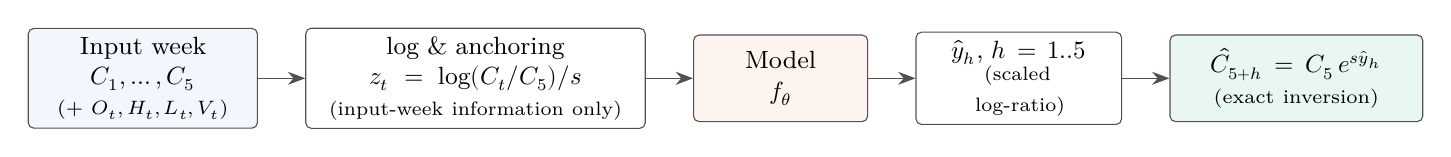
\begin{tikzpicture}[
  font=\small, >={Stealth[length=2.2mm]},
  box/.style={draw=ink2, rounded corners=2pt, fill=#1, minimum height=11mm, align=center, inner sep=3pt},
  box/.default=white]
\node[box=blue!6, text width=27mm] (in) {Input week\\ $C_1,\dots,C_5$\\ \scriptsize(+ $O_t,H_t,L_t,V_t$)};
\node[box=white, right=6mm of in, text width=41mm] (tr) {\mbox{log \& anchoring}\\ $z_t=\log(C_t/C_5)/s$\\ \scriptsize\mbox{(input-week information only)}};
\node[box=orange!8, right=6mm of tr, text width=20mm] (m) {Model\\ $f_\theta$};
\node[box=white, right=6mm of m, text width=24mm] (y) {$\hat y_h$, $h=1..5$\\ \scriptsize\mbox{(scaled}\\ \scriptsize\mbox{log-ratio)}};
\node[box=aqua!10, right=6mm of y, text width=30mm] (out) {$\hat C_{5+h}=C_5\,e^{s\hat y_h}$\\ \scriptsize(exact inversion)};
\draw[->, ink2] (in) -- (tr);
\draw[->, ink2] (tr) -- (m);
\draw[->, ink2] (m) -- (y);
\draw[->, ink2] (y) -- (out);
\end{tikzpicture}
\unskip}
  \caption{Common pipeline of all predictors: input transformation, model and exact inversion to prices.}
  \label{fig:pipeline}
\end{figure}

\subsection{Classical reference predictors}
All classical predictors are estimated on the training set only and evaluated with the same code as the neural models:
\begin{itemize}[leftmargin=*]
  \item \textbf{Persistence} (naive random-walk forecast): $\hat C_{5+h}=C_5$.
  \item \textbf{RW+drift}: $\log\hat C_{5+h}=\log C_5+h\hat\delta$, with $\hat\delta=\MuRetPct\%$ the mean daily return of the training set.
  \item \textbf{Linear trend (LS)}: a least-squares line fitted to the 5 values $\log C_t$ of the week and extrapolated (Lectures 4--5).
  \item \textbf{SES}: simple exponential smoothing $\hat m_t=\alpha x_t+(1-\alpha)\hat m_{t-1}$ of $\log C_t$ with the flat forecast $\hat m_5$; $\alpha=\SESalpha$ was chosen by grid search on the training set.
  \item \textbf{AR(4)-OLS}: a linear autoregression of order 4 on the daily returns, estimated by ordinary least squares (as \texttt{ar.ols} in the solved problems) and iterated recursively. It is the linear counterpart of the baseline; order 4 is the maximum allowed by the 5 prices of the week.
\end{itemize}

\subsection{Baseline: autoregressive Vanilla RNN (VRNN-AR)}
Following Lecture 1 \cite{elman1990,goodfellow2016}, the state is updated and the output computed as
\begin{equation}
  \mathbf h_t=\tanh(\mathbf U r_t+\mathbf W\mathbf h_{t-1}+\mathbf b),\qquad \hat r_{t+1}=\mathbf V\mathbf h_t+c,
\end{equation}
with $\mathbf h_1=\mathbf 0$ and $r_t=\log(C_t/C_{t-1})/s$. The input is univariate, because an autoregressive model must be able to feed its own output back as the next input. Training uses teacher forcing: from each window the inputs are $r_2,\dots,r_9$ and the one-step targets $r_3,\dots,r_{10}$. At forecast time (Fig.~\ref{fig:vrnn}) the network reads the 4 observed returns $r_2..r_5$ of the week and produces $\hat r_6$; then $\hat r_6$ is fed back as input to produce $\hat r_7$, and so on (closed loop). Finally $\yhat_h=\sum_{k\le h}\hat r_{5+k}$. The hyper-parameters (units $\in\{16,32,64\}$, layers $\in\{1,2\}$) are selected on the validation set \emph{according to the closed-loop 5-step forecast error}, not the one-step training error, so that the baseline is optimised for the actual task.

\begin{figure}[tbp]
  \centering
  \resizebox{0.95\linewidth}{!}{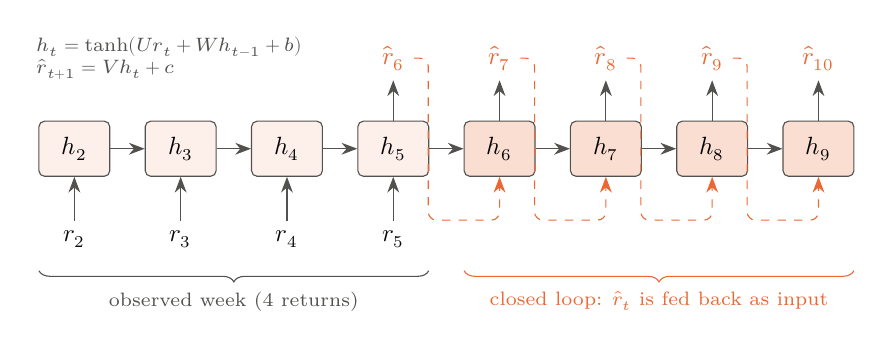
\begin{tikzpicture}[
  font=\small, >={Stealth[length=2mm]},
  cell/.style={draw=ink2, rounded corners=2pt, fill=orange!10, minimum width=9mm, minimum height=7mm},
  obs/.style={font=\small, text=ink},
  pred/.style={font=\small, text=orangeC}]
% observed part
\foreach \i/\lab in {1/2,2/3,3/4,4/5}{
  \node[cell] (h\i) at (1.35*\i,0) {$h_{\lab}$};
  \node[obs] (x\i) at (1.35*\i,-1.15) {$r_{\lab}$};
  \draw[->, ink2] (x\i) -- (h\i);
}
% closed-loop part
\foreach \i/\lab in {5/6,6/7,7/8,8/9}{
  \node[cell, fill=orange!22] (h\i) at (1.35*\i,0) {$h_{\lab}$};
}
\node[pred] (o4) at (1.35*4,1.15) {$\hat r_{6}$};
\foreach \i/\lab in {5/7,6/8,7/9,8/10}{\node[pred] (o\i) at (1.35*\i,1.15) {$\hat r_{\lab}$};}
\foreach \i in {4,...,8}{\draw[->, ink2] (h\i) -- (o\i);}
\foreach \i [evaluate=\i as \j using int(\i+1)] in {1,...,7}{\draw[->, ink2] (h\i) -- (h\j);}
% feedback arrows
\foreach \i [evaluate=\i as \j using int(\i+1)] in {4,...,7}{
  \draw[->, orangeC, dashed, rounded corners=3pt] (o\i.east) -- ++(0.18,0) |- ($(h\j.south)+(0,-0.55)$) -- (h\j.south);
}
\draw[decorate, decoration={brace, amplitude=4pt, mirror}, ink2] (0.9,-1.55) -- (5.85,-1.55)
  node[midway, below=4pt, font=\scriptsize] {observed week (4 returns)};
\draw[decorate, decoration={brace, amplitude=4pt, mirror}, orangeC] (6.3,-1.55) -- (11.25,-1.55)
  node[midway, below=4pt, font=\scriptsize] {closed loop: $\hat r_{t}$ is fed back as input};
\node[font=\scriptsize, ink2, align=left, anchor=west] at (0.75,1.15) {$h_t=\tanh(Ur_t+Wh_{t-1}+b)$\\ $\hat r_{t+1}=Vh_t+c$};
\end{tikzpicture}
\unskip}
  \caption{The autoregressive Vanilla RNN unrolled in time at forecast time. The 4 returns of the input week are read (left) and the next 5 are generated in closed loop (right, dashed arrows).}
  \label{fig:vrnn}
\end{figure}

\subsection{Encoder--decoder RNN with Bahdanau attention (Seq2Seq-Attn)}
Following Lecture 2 \cite{bahdanau2015}, the encoder is a bidirectional RNN (GRU \cite{cho2014}). Each day $j$ is represented by the concatenation $\mathbf h_j=[\overrightarrow{\mathbf h}_j;\overleftarrow{\mathbf h}_j]$. The decoder starts from $\mathbf s_0=\tanh(\mathbf W_s\overleftarrow{\mathbf h}_1)$ and for $i=1,\dots,5$ computes
\begin{align}
  e_{ij}&=\mathbf v_a^{\top}\tanh(\mathbf W_a\mathbf s_{i-1}+\mathbf U_a\mathbf h_j),\qquad
  \alpha_{ij}=\frac{\exp e_{ij}}{\sum_{k=1}^{5}\exp e_{ik}},\qquad
  \mathbf c_i=\sum_{j=1}^{5}\alpha_{ij}\mathbf h_j,\\
  \mathbf s_i&=f(\mathbf s_{i-1},\yhat_{i-1},\mathbf c_i),\qquad
  \yhat_i=g(\yhat_{i-1},\mathbf s_i,\mathbf c_i),
\end{align}
where $f$ is a GRU cell, $g$ a $\tanh$ hidden layer followed by a linear output, and $\yhat_0=z_5=0$. As stressed in the lecture, $\yhat_{i-1}$ injects autoregression into the decoder. Here the decoder is fed with its \emph{own} previous forecast during training as well (free-running): the whole model remains a single differentiable computational graph and there is no train/test mismatch (no exposure bias). Hyper-parameters: units $\in\{16,32,64\}$, dropout $\in\{0,0.1\}$.

\subsection{Encoder--decoder Transformer with horizon queries}
Following Lecture 3 \cite{vaswani2017}, each input day is linearly projected to dimension $d$, multiplied by $\sqrt d$, and the sinusoidal positional encoding is added. The encoder consists of $N$ blocks of multi-head self-attention and a feed-forward network (FFN), with residual connections and LayerNorm (post-LN, as in the original paper):
\begin{equation}
  \mathrm{Attention}(\mathbf Q,\mathbf K,\mathbf V)=\mathrm{softmax}\!\Big(\frac{\mathbf Q\mathbf K^{\top}}{\sqrt{d_k}}\Big)\mathbf V,\qquad
  \mathrm{MultiHead}=\mathrm{Concat}(\mathrm{head}_1,\dots,\mathrm{head}_H)\mathbf W^O .
\end{equation}
The decoder (Fig.~\ref{fig:transformer}) differs from the autoregressive decoder of the original Transformer in one respect: instead of the previous outputs, it receives 5 \emph{learned query vectors} $\mathbf q_1,\dots,\mathbf q_5\in\R^d$, one per horizon. The idea is borrowed from the object queries of DETR \cite{carion2020} and the ``generative'' decoder of the Informer \cite{zhou2021}. The queries go through self-attention among themselves without a causal mask, since all horizons are produced in parallel, and through encoder--decoder (cross) attention, in which $\mathbf K,\mathbf V$ come from the encoder. A linear head finally produces $\yhat_h$. Hence (i) there is neither error accumulation nor exposure bias, and (ii) each horizon ``decides'' which input days to attend to, with interpretable weights (Section~\ref{sec:analysis}). Hyper-parameters: $d\in\{16,32\}$, $N\in\{1,2\}$, 4 heads, FFN width $2d$, dropout 0.1.

\begin{figure}[tbp]
  \centering
  \resizebox{0.9\linewidth}{!}{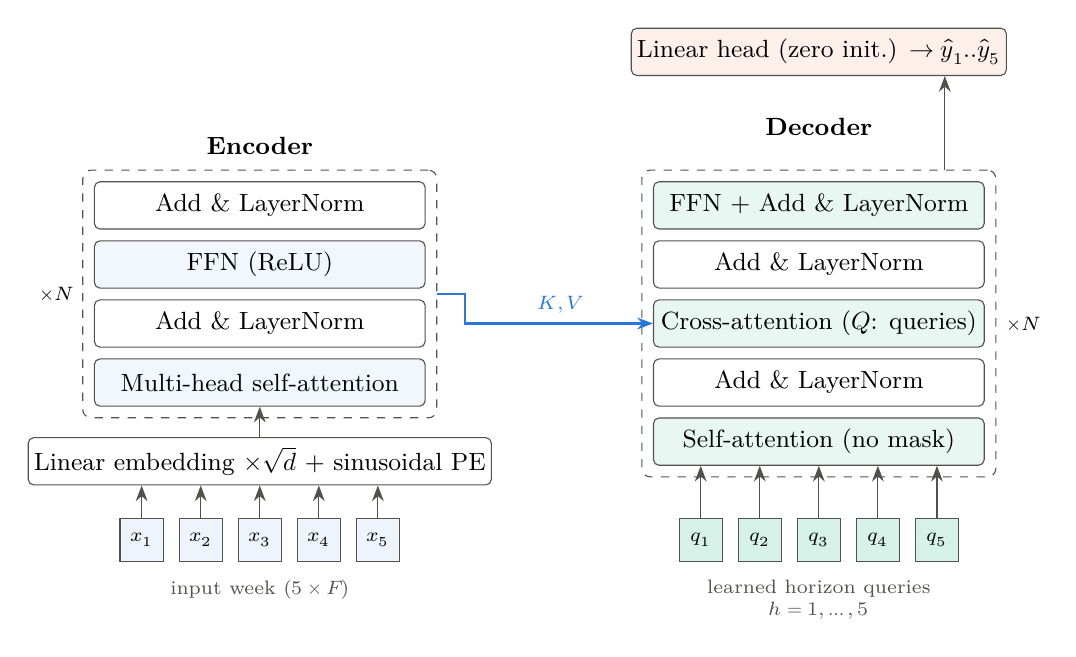
\begin{tikzpicture}[
  font=\small, >={Stealth[length=2mm]},
  blk/.style={draw=ink2, rounded corners=2pt, fill=#1, minimum width=42mm, minimum height=6mm, align=center, inner sep=2pt},
  blk/.default=white,
  tok/.style={draw=ink2, fill=blue!8, minimum width=5.5mm, minimum height=5.5mm, inner sep=0pt, font=\scriptsize},
  qry/.style={draw=ink2, fill=aqua!18, minimum width=5.5mm, minimum height=5.5mm, inner sep=0pt, font=\scriptsize}]
% ---------------- encoder
\foreach \i in {1,...,5}{\node[tok] (t\i) at (0.75*\i-0.15,0) {$x_\i$};}
\node[font=\scriptsize, ink2, below=1mm of t3] {input week ($5\times F$)};
\node[blk] (emb) at (2.1,1.0) {Linear embedding $\times\sqrt{d}$ + sinusoidal PE};
\node[blk=blue!6] (sa) at (2.1,2.0) {Multi-head self-attention};
\node[blk] (an1) at (2.1,2.75) {Add \& LayerNorm};
\node[blk=blue!6] (ff) at (2.1,3.5) {FFN (ReLU)};
\node[blk] (an2) at (2.1,4.25) {Add \& LayerNorm};
\node[draw=ink2, dashed, rounded corners=3pt, fit=(sa)(an2), inner sep=4pt, label={[font=\scriptsize]left:$\times N$}] (encbox) {};
\node[font=\small\bfseries] at (2.1,5.0) {Encoder};
\foreach \i in {1,...,5}{\draw[->, ink2] (t\i.north) -- (t\i.north |- emb.south);}
\draw[->, ink2] (emb) -- (sa);
% ---------------- decoder
\foreach \i in {1,...,5}{\node[qry] (q\i) at (6.95+0.75*\i,0) {$q_\i$};}
\node[font=\scriptsize, ink2, below=1mm of q3, align=center] {learned horizon queries\\ $h=1,\dots,5$};
\node[blk=aqua!10] (dsa) at (9.2,1.25) {Self-attention (no mask)};
\node[blk] (dan1) at (9.2,2.0) {Add \& LayerNorm};
\node[blk=aqua!10] (ca) at (9.2,2.75) {Cross-attention ($Q$: queries)};
\node[blk] (dan2) at (9.2,3.5) {Add \& LayerNorm};
\node[blk=aqua!10] (dff) at (9.2,4.25) {FFN + Add \& LayerNorm};
\node[draw=ink2, dashed, rounded corners=3pt, fit=(dsa)(dff), inner sep=4pt, label={[font=\scriptsize]right:$\times N$}] (decbox) {};
\node[font=\small\bfseries] at (9.2,5.25) {Decoder};
\foreach \i in {1,...,5}{\draw[->, ink2] (q\i.north) -- (q\i.north |- dsa.south);}
\node[blk=orange!10, minimum width=42mm] (head) at (9.2,6.2) {Linear head (zero init.) $\rightarrow \hat y_1..\hat y_5$};
\draw[->, ink2] ($(decbox.north)+(1.6,0)$) -- ($(head.south)+(1.6,0)$);
% memory -> cross attention
\draw[->, blueC, thick] (encbox.east) -- ++(0.35,0) |- (ca.west) node[pos=0.75, above, font=\scriptsize] {$K,V$};
\end{tikzpicture}
\unskip}
  \caption{The encoder--decoder Transformer with learned horizon queries. The 5 horizons are decoded in parallel (non-autoregressively).}
  \label{fig:transformer}
\end{figure}

\subsection{Additional model for the ablation study: VRNN-Direct}
The same Vanilla RNN cell reads the week and its final state is mapped directly to the 5 horizons. Comparing VRNN-AR with VRNN-Direct isolates the effect of the forecasting \emph{strategy}; comparing VRNN-Direct, Seq2Seq-Attn and the Transformer isolates the effect of the \emph{attention mechanism}. Every direct model is also trained with both feature sets, which isolates the effect of the \emph{features}.

\subsection{Common design choices}
\label{sec:common}
\begin{itemize}[leftmargin=*]
  \item \textbf{Zero-initialised head:} in every network the last linear layer is initialised to zero. At the start of training each network is therefore exactly the persistence forecast and moves away from it only as far as the data support. This is a natural inductive bias for near-random walks.
  \item \textbf{Loss function:} MSE on $y_h$, whose minimiser is the conditional mean of the log-change.
  \item \textbf{Ensemble:} the final predictor of each family is the average of 5 networks trained with different seeds \cite{lakshminarayanan2017}. This reduces the variance due to initialisation, which matters when the signal is weak.
\end{itemize}

% ======================================================================== 5
\section{Experimental protocol}
\label{sec:exp}

\subsection{Training}
We use Keras~3 / TensorFlow (CPU), the AdamW optimiser \cite{loshchilov2019} ($\eta=10^{-3}$, weight decay $10^{-4}$, gradient clipping 1.0), batch size 128 and at most 150 epochs. Early stopping monitors the MSE of the \emph{5-step forecast} on the validation set, with a patience of 15 epochs and restoration of the best weights. The criterion is the same for all models and, for VRNN-AR, is computed in closed loop. Determinism is ensured with fixed seeds and \texttt{enable\_op\_determinism}.

\subsection{Selection of hyper-parameters and of the final model}
Each grid configuration is trained with 2 seeds and the one with the lowest mean validation MSE is selected (Table~\ref{tab:configs}). The selected configurations are then trained with 5 new seeds. \textbf{The proposed model was defined in advance} as the attention-based candidate (Seq2Seq-Attn or Transformer, with close or OHLCV input) with the lowest validation MSE of its ensemble. The test set was used \emph{once}, after the selection.

\begin{table}[t]
\centering\small
\caption{Selected hyper-parameters per model family and feature set (grid $\times$ 2 seeds; criterion: validation forecast MSE). $d$: model dimension, $N$: number of blocks. ``Epoch'': mean best-validation epoch over the 5 final training runs.}
\label{tab:configs}
\begin{tabular}{llllrrr}
\toprule
Model & Input & Selected configuration & Params & Configs & MSE$_{\text{val}}$ & Epoch\\
\midrule
\eng{VRNN-AR} & \eng{returns} & \eng{layers=2, units=32} & 3,201 & 6 & 1.8581 & 6.0 \\
\eng{VRNN-Direct} & \eng{close} & \eng{layers=1, units=16} & 373 & 6 & 1.8454 & 86.8 \\
\eng{VRNN-Direct} & \eng{ohlcv} & \eng{layers=1, units=32} & 1,381 & 6 & 1.8617 & 8.4 \\
\eng{Seq2Seq-Attn} & \eng{close} & \eng{units=64, dropout=0.1} & 92,161 & 6 & 1.8351 & 29.0 \\
\eng{Seq2Seq-Attn} & \eng{ohlcv} & \eng{units=64, dropout=0.1} & 93,697 & 6 & 1.8548 & 6.6 \\
\eng{Transformer} & \eng{close} & \eng{d=16, N=1, heads=4, dropout=0.1} & 5,697 & 4 & 1.8329 & 56.0 \\
\eng{Transformer} & \eng{ohlcv} & \eng{d=16, N=1, heads=4, dropout=0.1} & 5,761 & 4 & 1.8310 & 21.0 \\
\bottomrule
\end{tabular}
\end{table}


\subsection{Metrics}
With $e=\hat C-C$ we report, per horizon and pooled:
\begin{itemize}[leftmargin=*]
  \item MAE and RMSE in €, and $\mathrm{MAPE}=100\cdot\overline{|e|/C}$. Since MAE and RMSE in € are dominated by the expensive stocks, MAPE is the primary metric.
  \item $\mathrm{RMSE}_{\log}=100\sqrt{\overline{(\log\hat C-\log C)^2}}$, a scale-free error in percentage points, and Theil's $U=\mathrm{RMSE}_{\log}/\mathrm{RMSE}_{\log}^{\text{persistence}}$ \cite{theil1966}; $U<1$ means a better forecast than the naive one.
  \item DA (directional accuracy): the percentage of windows in which the forecast direction ($\hat C_{5+h}$ versus $C_5$) matches the actual one. It is undefined for persistence.
\end{itemize}

\subsection{Diebold--Mariano test}
To compare two predictors $A$ and $B$ we apply the Diebold--Mariano test \cite{diebold1995} with $H_0$: equal expected loss. The loss is the squared log-error, averaged over the 5 horizons or taken per horizon. Two adjustments are needed for our data: (a) the loss differential $d$ is first averaged across stocks for each forecast date, which removes the cross-sectional dependence; (b) the long-run variance of $d_t$ is estimated with a Newey--West kernel \cite{newey1987} with 9 lags, covering the overlap of consecutive 10-day windows (a conservative choice). The Harvey--Leybourne--Newbold small-sample correction \cite{harvey1997} is applied, with a $t_{T-1}$ reference distribution.

% ======================================================================== 6
\section{Results}
\label{sec:results}

\subsection{Selection of the proposed model (validation set)}
On the validation set, persistence has an MSE of \ValPersMSE{} in the scaled space. Among the four attention-based candidates, the lowest MSE (\ValPropMSE, $-$\ValPropGain\% relative to persistence) was achieved by \textbf{\PropName}: an encoder--decoder RNN with Bahdanau attention, 64 units, dropout 0.1, and the 5 closing prices as input. The VRNN-AR baseline obtained \ValVrnnMSE{} ($-$\ValVrnnGain\%). All validation figures are listed in Table~\ref{tab:val} of the Appendix. \textbf{\PropName{} is the proposed predictor}; it was selected before any evaluation on the test set.

\subsection{Main results (test set)}
\begin{table}[t]
\centering\small
\caption{Test set (5 stocks, \Ntest{} windows): forecast errors pooled over all horizons ($h=1..5$). Neural models are 5-seed ensembles; the last column gives the MAPE of the individual seeds (mean $\pm$ s.d.). Bold: best value per column; $^{\star}$: proposed model (selected on the validation set).}
\label{tab:main}
\footnotesize
\setlength{\tabcolsep}{4pt}
\begin{tabular}{lrrrrrrr}
\toprule
Model & MAPE (\%) & RMSE$_{\log}$ (\%) & Theil $U$ & MAE (€) & RMSE (€) & DA (\%) & MAPE, seeds\\
\midrule
\eng{Persistence} & 2.275 & 3.185 & 1.0000 & 0.2581 & 0.3822 & — & — \\
\eng{RW+drift} & 2.275 & 3.174 & 0.9964 & 0.2576 & 0.3814 & 53.4 & — \\
\eng{Linear trend (LS)} & 3.257 & 4.596 & 1.4429 & 0.3679 & 0.5470 & 49.7 & — \\
\eng{SES} & 2.274 & 3.185 & 0.9999 & 0.2581 & 0.3821 & 49.8 & — \\
\eng{AR(4)-OLS} & 2.274 & 3.173 & 0.9962 & 0.2575 & 0.3811 & 52.6 & — \\
\midrule
\eng{VRNN-AR} & 2.265 & 3.160 & 0.9921 & 0.2565 & 0.3794 & 53.6 & 2.270\,$\pm$\,0.005 \\
\eng{VRNN-Direct [close]} & 2.258 & 3.145 & 0.9875 & 0.2558 & 0.3776 & 53.7 & 2.261\,$\pm$\,0.002 \\
\eng{VRNN-Direct [OHLCV]} & 2.262 & 3.156 & 0.9907 & 0.2563 & 0.3792 & 54.0 & 2.265\,$\pm$\,0.004 \\
\rowcolor{best}\eng{Seq2Seq-Attn [close]}$^{\star}$ & \textbf{2.245} & \textbf{3.129} & \textbf{0.9823} & \textbf{0.2545} & \textbf{0.3760} & 53.7 & 2.249\,$\pm$\,0.003 \\
\eng{Seq2Seq-Attn [OHLCV]} & 2.247 & 3.136 & 0.9847 & 0.2549 & 0.3774 & \textbf{54.1} & 2.256\,$\pm$\,0.004 \\
\eng{Transformer [close]} & 2.258 & 3.151 & 0.9891 & 0.2559 & 0.3786 & 53.4 & 2.259\,$\pm$\,0.002 \\
\eng{Transformer [OHLCV]} & 2.261 & 3.154 & 0.9902 & 0.2562 & 0.3790 & 53.5 & 2.266\,$\pm$\,0.006 \\
\bottomrule
\end{tabular}
\end{table}


Table~\ref{tab:main} summarises the results on the 5 unseen test stocks.
\begin{itemize}[leftmargin=*]
  \item \textbf{The proposed predictor is the best on every error metric.} Its MAPE is \PropMAPE\%, against \PersMAPE\% for persistence and \VrnnMAPE\% for the baseline. Its Theil index is $U=\PropU$, i.e.\ an MSE reduction of \PropGain\% relative to persistence. The reduction is \VrnnGain\% for VRNN-AR and only \DriftGain\% and \ArGain\% for the classical RW+drift and AR(4)-OLS.
  \item \textbf{The ranking is consistent between validation and test.} \PropName{} is first on both sets, all neural models outperform all classical ones, and the classical models are practically equivalent to persistence. The selection is therefore not a chance result of overfitting the validation set.
  \item \textbf{The ensemble helps:} the MAPE of the individual seeds of the proposed model is \PropSeedMAPE$\pm$\PropSeedMAPEsd\%, whereas the ensemble reaches \PropMAPE\%. Even the worst single seed is better than every non-neural model.
  \item \textbf{Linear-trend extrapolation} (LS) is clearly worse than persistence ($U=\TrendU$). This agrees with the slightly negative autocorrelation: short-term ``trends'' do not persist.
  \item \textbf{Directional accuracy:} all models have a DA of 53--54\%. This is practically equal to the share of upward moves in the period (RW+drift, which always forecasts a rise: \DriftDA\%). The direction of next week's move is \emph{not} predicted materially better than the base rate.
\end{itemize}

\begin{figure}[tbp]
  \centering
  \includegraphics[width=\linewidth]{\figdir/res_examples.pdf}
  \caption{Example forecasts on the 5 test stocks (last 12 non-overlapping weeks). Each coloured segment starts from the last known price $C_5$ and shows the forecast of the next 5 sessions.}
  \label{fig:examples}
\end{figure}

\subsection{Per horizon}
\begin{figure}[tbp]
  \centering
  \includegraphics[width=\linewidth]{\figdir/res_horizon.pdf}
  \caption{(a) MAPE per horizon: the error grows roughly as $\sqrt h$, as a random walk implies, and the curves of all models almost coincide. (b) Theil's $U$ reveals the relative differences ($U<1$: better than persistence).}
  \label{fig:horizon}
\end{figure}
\begin{table}[t]
\centering\small
\caption{Test set: MAPE (\%) and Theil's $U$ per forecast horizon $h$ (sessions).}
\label{tab:horizon}
\setlength{\tabcolsep}{3.6pt}
\begin{tabular}{l*{5}{r}|*{5}{r}}
\toprule
& \multicolumn{5}{c|}{MAPE (\%)} & \multicolumn{5}{c}{Theil $U$}\\
Model & $h{=}1$ & 2 & 3 & 4 & 5 & $h{=}1$ & 2 & 3 & 4 & 5\\
\midrule
\eng{Persistence} & 1.34 & 1.92 & 2.35 & 2.72 & 3.04 & — & — & — & — & — \\
\eng{RW+drift} & 1.35 & 1.92 & 2.35 & 2.72 & 3.04 & 0.999 & 0.998 & 0.997 & 0.996 & 0.995 \\
\eng{AR(4)-OLS} & 1.35 & 1.92 & 2.35 & 2.72 & 3.04 & 0.999 & 0.998 & 0.997 & 0.996 & 0.995 \\
\eng{VRNN-AR} & 1.34 & 1.91 & 2.34 & 2.71 & 3.03 & 0.991 & 0.992 & 0.992 & 0.993 & 0.992 \\
\eng{VRNN-Direct [OHLCV]} & 1.34 & 1.90 & 2.33 & 2.71 & 3.03 & 0.991 & 0.990 & 0.990 & 0.991 & 0.991 \\
\rowcolor{best}\eng{Seq2Seq-Attn [close]}$^{\star}$ & 1.33 & 1.89 & 2.32 & 2.68 & 3.00 & 0.976 & 0.983 & 0.984 & 0.983 & 0.982 \\
\eng{Seq2Seq-Attn [OHLCV]} & 1.33 & 1.89 & 2.32 & 2.69 & 3.00 & 0.982 & 0.985 & 0.985 & 0.985 & 0.985 \\
\eng{Transformer [close]} & 1.34 & 1.90 & 2.33 & 2.70 & 3.02 & 0.989 & 0.990 & 0.991 & 0.989 & 0.988 \\
\eng{Transformer [OHLCV]} & 1.34 & 1.91 & 2.34 & 2.70 & 3.02 & 0.994 & 0.991 & 0.990 & 0.990 & 0.990 \\
\bottomrule
\end{tabular}
\end{table}


The absolute error is dominated by market volatility. The MAPE of persistence grows from \PersMAPEhOne\% ($h=1$) to \PersMAPEhFive\% ($h=5$), and all models follow the same $\propto\sqrt h$ curve (Fig.~\ref{fig:horizon}a, Table~\ref{tab:horizon}). In relative terms (Fig.~\ref{fig:horizon}b), the proposed model has its largest gain at $h=1$ ($U=\PropUhOne$) and keeps $U\approx0.98$ at every horizon. VRNN-AR starts at $U=\VrnnUhOne$ and stays close to $0.99$. The linear models (RW+drift, AR(4)-OLS) improve slightly with the horizon, because their gain comes almost exclusively from the drift, which accumulates linearly.

\subsection{Statistical significance}
\begin{table}[t]
\centering\small
\caption{Diebold--Mariano tests on the test set (HLN correction, Newey--West with 9 lags, losses averaged across stocks per forecast date). A negative statistic means that the row model is more accurate than the reference model of the column. Bold: $p<0.05$.}
\label{tab:dm}
\footnotesize
\setlength{\tabcolsep}{2.6pt}
\begin{tabular}{l*{10}{r}}
\toprule
& \multicolumn{6}{c}{vs.\ Persistence} & \multicolumn{2}{c}{vs.\ VRNN-AR} & \multicolumn{2}{c}{vs.\ \eng{Seq2Seq-Attn [close]}}\\
\cmidrule(lr){2-7}\cmidrule(lr){8-9}\cmidrule(lr){10-11}
& \multicolumn{2}{c}{all $h$} & \multicolumn{2}{c}{$h=1$} & \multicolumn{2}{c}{$h=5$} & \multicolumn{2}{c}{all $h$} & \multicolumn{2}{c}{all $h$}\\
Model & DM & $p$ & DM & $p$ & DM & $p$ & DM & $p$ & DM & $p$\\
\midrule
\eng{RW+drift} & -0.75 & 0.455 & -0.70 & 0.486 & -0.77 & 0.442 & \textbf{2.22} & 0.027 & \textbf{1.98} & 0.049 \\
\eng{Linear trend (LS)} & \textbf{6.76} & <0.001 & \textbf{8.56} & <0.001 & \textbf{6.34} & <0.001 & \textbf{6.72} & <0.001 & \textbf{6.50} & <0.001 \\
\eng{SES} & -0.17 & 0.866 & 0.41 & 0.680 & 0.04 & 0.972 & 1.64 & 0.101 & \textbf{2.30} & 0.022 \\
\eng{AR(4)-OLS} & -0.79 & 0.432 & -0.64 & 0.524 & -0.74 & 0.460 & \textbf{2.07} & 0.039 & 1.90 & 0.058 \\
\eng{VRNN-AR} & -1.67 & 0.097 & \textbf{-2.35} & 0.019 & -1.25 & 0.211 & — & — & 1.79 & 0.074 \\
\eng{VRNN-Direct [close]} & -1.96 & 0.050 & \textbf{-2.00} & 0.046 & -1.65 & 0.100 & -1.41 & 0.159 & 1.81 & 0.070 \\
\eng{VRNN-Direct [OHLCV]} & -1.77 & 0.076 & \textbf{-2.54} & 0.011 & -1.34 & 0.180 & -0.71 & 0.477 & 1.53 & 0.127 \\
\rowcolor{best}\eng{Seq2Seq-Attn [close]}$^{\star}$ & \textbf{-2.30} & 0.022 & -1.79 & 0.074 & \textbf{-2.07} & 0.039 & -1.79 & 0.074 & — & — \\
\eng{Seq2Seq-Attn [OHLCV]} & -1.91 & 0.056 & \textbf{-2.20} & 0.028 & -1.63 & 0.103 & -1.39 & 0.164 & 0.74 & 0.459 \\
\eng{Transformer [close]} & -1.84 & 0.066 & \textbf{-2.07} & 0.039 & -1.62 & 0.105 & -1.05 & 0.296 & 1.84 & 0.067 \\
\eng{Transformer [OHLCV]} & -1.62 & 0.105 & \textbf{-2.26} & 0.024 & -1.39 & 0.164 & -0.73 & 0.464 & 1.66 & 0.098 \\
\bottomrule
\end{tabular}
\end{table}


The Diebold--Mariano tests (Table~\ref{tab:dm}) show that:
\begin{enumerate}[leftmargin=*]
  \item \PropName{} is the \textbf{only} model that significantly outperforms persistence at the 5\% level over all horizons jointly ($\mathrm{DM}=\PropDMpers$, $p=\PropPpers$) and at $h=5$ ($p=\PropPpersHFive$). It also significantly outperforms RW+drift ($p=\DriftPprop$). Against AR(4)-OLS ($p=\ArPprop$) and VRNN-AR ($p=\PropPvrnn$) its advantage is marginal, at the 10\% level.
  \item The VRNN-AR baseline does not differ significantly from persistence over all horizons jointly ($p=\VrnnPpers$). It is, however, better at $h=1$ ($p=\VrnnPpersHOne$) and significantly better than the linear RW+drift ($p=\VrnnPdrift$) and AR(4)-OLS ($p=\VrnnPar$). The non-linearity of the RNN pays off, but its gain is lost at longer horizons of the closed loop (Section~\ref{sec:analysis}).
  \item The classical RW+drift, SES and AR(4)-OLS are statistically indistinguishable from persistence ($p>0.4$), as expected for a near-random walk.
\end{enumerate}
The significance levels are conservative, because the dependence between stocks is removed by averaging per date and 9 HAC lags are used. No multiple-comparison correction was applied: a single comparison was defined in advance (proposed model versus persistence/baseline), and the remaining ones are exploratory.

\subsection{Robustness: per stock and calendar weeks}
\begin{table}[t]
\centering\small
\caption{Robustness checks on the test set: MAPE (\%) per stock and under the strict calendar-week protocol (input Monday--Friday, target the following Monday--Friday).}
\label{tab:robust}
\setlength{\tabcolsep}{4pt}
\begin{tabular}{l*{5}{r}}
\toprule
Stock & \eng{Persistence} & \eng{RW+drift} & \eng{AR(4)-OLS} & \eng{VRNN-AR} & \eng{Seq2Seq-Attn [close]}$^{\star}$\\
\midrule
\#8 & 2.915 & 2.898 & 2.912 & 2.896 & \textbf{2.860} \\
\#11 & 2.029 & 2.008 & 2.006 & 1.999 & \textbf{1.976} \\
\#13 & 1.836 & 1.849 & 1.846 & 1.842 & \textbf{1.832} \\
\#15 & 2.699 & 2.703 & 2.695 & 2.682 & \textbf{2.655} \\
\#22 & \textbf{1.895} & 1.918 & 1.912 & 1.908 & 1.901 \\
\midrule
\makecell[l]{Calendar\\ weeks (330)} & \textbf{2.193} & 2.211 & 2.216 & 2.217 & 2.209 \\
\quad \eng{Theil} $U$ & — & 1.0005 & 1.0030 & 1.0027 & 0.9994 \\
\bottomrule
\end{tabular}
\end{table}


\paragraph{Per stock}
Table~\ref{tab:robust} shows that the proposed model has a lower MAPE than persistence for \PropBeatsPersStocks/\NtestStocks{} stocks and lower than VRNN-AR for \PropBeatsVrnnStocks/\NtestStocks, so the improvement is not due to a single stock. The only exception is \#22, the only test stock with a \emph{declining} path over the two years ($-21\%$). There persistence wins marginally, which is expected since all trained models have learned a positive drift.

\paragraph{Calendar weeks}
On the strict subset with a Monday--Friday input and the following Monday--Friday as target (\NcalTest{} windows, \CwWeeks{} weeks), \textbf{no model differs significantly from persistence}: $U=\CwPropU$ ($p=\CwPropP$) for the proposed model and $U=\CwVrnnU$ ($p=\CwVrnnP$) for VRNN-AR. This subset is about $1/7$ of the test set. Given the observed dispersion of the losses, an MSE improvement of 2--4\% cannot be detected with 66 independent weeks. The result confirms that the true predictive margin is small and requires large samples to be measured reliably. We report it explicitly so that the practical importance of the gains is not overstated.

\subsection{Ablation study}
The pairwise comparisons in Table~\ref{tab:main} answer three questions:
\begin{itemize}[leftmargin=*]
  \item \textbf{Strategy (recursive versus direct):} with the same Vanilla RNN cell, direct forecasting improves $U$ from \VrnnU{} to \DirCloseU{}. The improvement has the right sign but is not significant ($p=\DirectPvrnn$).
  \item \textbf{Attention mechanism:} with the same close input, adding Bahdanau attention in an encoder--decoder improves $U$ from \DirCloseU{} (VRNN-Direct) to \SsCloseU. By contrast, the Transformer ($U=\TrCloseU$) does not improve on the simple VRNN-Direct. With only 5 time steps, the Transformer's advantage in long-range dependencies cannot be exploited, whereas the recurrent encoder provides a useful inductive bias for temporal order. This agrees with the literature, where simpler models often compete with Transformers on time series \cite{zeng2023}.
  \item \textbf{Features (close versus OHLCV):} OHLCV did \emph{not} help any architecture ($U$: \SsOhlcvU{} vs.\ \SsCloseU{} for Seq2Seq-Attn, \TrOhlcvU{} vs.\ \TrCloseU{} for the Transformer, \DirOhlcvU{} vs.\ \DirCloseU{} for VRNN-Direct). The OHLCV models stop much earlier (Table~\ref{tab:configs}), i.e.\ they overfit faster. The intraday features carry mostly \emph{volatility} information, which does not improve the forecast of the \emph{mean} under an MSE loss. The only hint of a benefit is a slightly higher DA (\SsOhlcvDA\%).
\end{itemize}

\subsection{What the models learned}
\label{sec:analysis}

\begin{figure}[tbp]
  \centering
  \includegraphics[width=\linewidth]{\figdir/res_attention.pdf}
  \caption{Mean attention weights on the test set (5 seeds, all windows): for each horizon $h$ (rows), the attention paid to each day of the input week (columns; $t$ = last day). A uniform distribution corresponds to $0.20$.}
  \label{fig:attention}
\end{figure}

\paragraph{Attention weights}
In the proposed model (Fig.~\ref{fig:attention}a) attention clearly \emph{decays into the past}: the last day receives a weight of \AttLastMin--\AttLastMax, increasing with the horizon, the day before \AttPrev, and the first two days only \AttFirstTwo{} on average. The pattern resembles the exponentially decaying weights $\alpha(1-\alpha)^j$ of exponential smoothing (Lectures 4--5), except that here the weights depend on the input and are learned from the data. In the Transformer (Fig.~\ref{fig:attention}b) attention is almost uniform, with a mild preference for the last day (\AttTrLast{} on average): the model essentially ``summarises'' the week.

\begin{figure}[tbp]
  \centering
  \includegraphics[width=\linewidth]{\figdir/res_exposure_bias.pdf}
  \caption{VRNN-AR on the test set. (a) MSE of the daily-return forecast $\hat r_{5+k}$ relative to the zero forecast. In closed loop the RNN is fed with its own forecasts; in the teacher-forcing diagnostic it is fed with the true returns, which are not available in practice. (b) The dispersion of the forecasts shrinks in closed loop.}
  \label{fig:exposure}
\end{figure}

\paragraph{Exposure bias of the baseline}
Fig.~\ref{fig:exposure} explains why the autoregressive RNN loses its advantage after the first step. When it receives the true returns, it keeps, and even slightly improves, its predictive ability at every step (the MSE ratio falls from \EbClOne{} to \EbTfFive). In closed loop the ratio rises from \EbClOne{} ($k=1$) to \EbClFive{} ($k=5$) and the dispersion of the forecasts shrinks. Its own forecasts, much ``smoother'' than the true returns, carry no new information, and the recursion converges to a fixed point close to the drift. This is exactly the exposure-bias phenomenon \cite{bengio2015}. The proposed model avoids it because it is trained in the same (free-running) mode in which it is used.

\begin{figure}[tbp]
  \centering
  \includegraphics[width=0.92\linewidth]{\figdir/res_learning_curves.pdf}\\[4pt]
  \includegraphics[width=0.46\linewidth]{\figdir/res_pred_vs_actual.pdf}
  \caption{Top: validation forecast MSE per epoch (5 seeds; dot: best epoch) for (a) the baseline and (b) the proposed model. Bottom: forecast versus realised 5-day return on the test set.}
  \label{fig:learning}
\end{figure}

\paragraph{Training dynamics}
For VRNN-AR the validation error is minimised within the first epochs (best epochs: \VrnnBestEpochs) and then increases (Fig.~\ref{fig:learning}, top): the model quickly learns the drift and then starts fitting noise. The proposed model improves steadily for 26--36 epochs (\PropBestEpochs), with dropout and early stopping limiting overfitting.

\paragraph{Forecast behaviour}
The mean forecast 5-day return of the proposed model is \PropMeanFive\%, close to the actual mean (\ActualMeanFive\%) and to the drift (\DriftMeanFive\%). However, the standard deviation of its forecasts is only \PropSdFive\%, against \ActualSdFive\% for the actual returns (Fig.~\ref{fig:learning}, bottom). The forecasts are thus about 9 times more ``compressed'' than reality, as expected from a good conditional-mean estimate when the signal is weak. The forecast--realisation correlation is $\rho=\PropCorrFive$, almost twice that of VRNN-AR ($\rho=\VrnnCorrFive$). It corresponds to $R^2\approx3\%$, consistent with the \PropGain\% MSE reduction.

% ======================================================================== 7
\FloatBarrier
\section{Discussion}
\label{sec:discussion}

\paragraph{Interpretation}
The results agree with the exploratory analysis. Returns are close to white noise (Ljung--Box), so the mean of next week is barely predictable from the current week, and all models produce forecasts close to the last price (Fig.~\ref{fig:examples}). The question is therefore not whether a model ``predicts the market'', but whether it extracts the small available signal \emph{systematically} and \emph{without overfitting}. The proposed model does so. It is the best on validation and test and at every horizon, it beats persistence for \PropBeatsPersStocks/\NtestStocks{} stocks, and it is the only model with a statistically significant ($\alpha=5\%$) advantage over persistence. The gain (\PropGain\% in MSE) is small in absolute terms but realistic; a much larger gain on such data would indicate leakage.

\paragraph{Why Bahdanau attention and not the Transformer}
The input week has only 5 points, so the Transformer's main advantage, connecting distant positions at constant cost (Lecture 3), cannot be exploited. The bidirectional recurrent encoder builds temporal order into the architecture, whereas the Transformer has to learn it from the positional encoding. Moreover, the Seq2Seq-Attn decoder is ``mildly'' autoregressive, since $\yhat_{i-1}$ enters $f$ and $g$; because it is trained in free-running mode, it exploits the consistency between horizons without exposure bias.

\paragraph{Limitations}
\begin{itemize}[leftmargin=*]
  \item \textbf{Same time period in all sets.} The split by stock means that the evaluation measures generalisation to \emph{new stocks}, not to a \emph{new period}. Common market shocks also appear in training; this is why we avoided calendar features (Section~\ref{sec:data}). The positive drift learned by all models is specific to this bullish period and would work against them in a falling market (see stock \#22).
  \item \textbf{Statistical power.} The \Ntest{} test windows overlap and come from 5 stocks, so the effective sample size is much smaller, as the calendar-week subset showed.
  \item \textbf{Point forecasts.} The ACF of the squared returns shows that \emph{volatility} is strongly predictable. A probabilistic forecast (e.g.\ quantiles or a full distribution) would have more practical value than a point forecast.
  \item \textbf{Economic significance.} DA does not materially exceed the base rate of upward moves. Without transaction costs and risk management, the results do not constitute a trading strategy.
\end{itemize}

\paragraph{Future work}
(i) Out-of-time (walk-forward) evaluation with newer data. (ii) Probabilistic forecasts with a quantile loss or a volatility model. (iii) Exogenous variables (market index, sector), if allowed by the problem definition. (iv) Robust losses (Huber) for the heavy tails.

% ======================================================================== 8
\section{Conclusions}
We designed, implemented and rigorously evaluated a predictor of next-week closing prices for stocks of the Athens Stock Exchange. The predictor is an encoder--decoder RNN with Bahdanau attention whose input is the 5 closing prices of the current week; it was selected on the validation set among four attention-based models. On the 5 unseen test stocks it:
\begin{itemize}[leftmargin=*]
  \item achieved a MAPE of \PropMAPE\%, against \VrnnMAPE\% for the required baseline (autoregressive Vanilla RNN) and \PersMAPE\% for the naive forecast;
  \item reduced the MSE by \PropGain\% relative to the naive forecast, with a statistically significant difference ($p=\PropPpers$), and was better than the baseline at every horizon and for every stock (marginal significance, $p=\PropPvrnn$).
\end{itemize}
The analysis showed three things: (a) the recursive strategy of the baseline suffers from exposure bias; (b) attention learns an interpretable pattern of weights decaying into the past, akin to exponential smoothing; (c) the additional OHLCV features increase overfitting without any benefit. The realistic size of the gain, and its absence in smaller subsets, reflect the nature of stock prices as near-random walks.


% ======================================================================== refs
\begin{thebibliography}{99}\small
\bibitem{bahdanau2015} D. Bahdanau, K. Cho, Y. Bengio, ``Neural machine translation by jointly learning to align and translate,'' \emph{ICLR}, 2015.
\bibitem{vaswani2017} A. Vaswani \emph{et al.}, ``Attention is all you need,'' \emph{NIPS}, 2017.
\bibitem{goodfellow2016} I. Goodfellow, Y. Bengio, A. Courville, \emph{Deep Learning}, MIT Press, 2016, ch.~10.
\bibitem{elman1990} J. L. Elman, ``Finding structure in time,'' \emph{Cognitive Science}, 14(2):179--211, 1990.
\bibitem{cho2014} K. Cho \emph{et al.}, ``Learning phrase representations using RNN encoder--decoder for statistical machine translation,'' \emph{EMNLP}, 2014.
\bibitem{williams1989} R. J. Williams, D. Zipser, ``A learning algorithm for continually running fully recurrent neural networks,'' \emph{Neural Computation}, 1(2):270--280, 1989.
\bibitem{bengio2015} S. Bengio, O. Vinyals, N. Jaitly, N. Shazeer, ``Scheduled sampling for sequence prediction with recurrent neural networks,'' \emph{NIPS}, 2015.
\bibitem{bentaieb2012} S. Ben Taieb, G. Bontempi, A. F. Atiya, A. Sorjamaa, ``A review and comparison of strategies for multi-step ahead time series forecasting based on the NN5 forecasting competition,'' \emph{Expert Systems with Applications}, 39(8):7067--7083, 2012.
\bibitem{carion2020} N. Carion \emph{et al.}, ``End-to-end object detection with transformers,'' \emph{ECCV}, 2020.
\bibitem{zhou2021} H. Zhou \emph{et al.}, ``Informer: Beyond efficient transformer for long sequence time-series forecasting,'' \emph{AAAI}, 2021.
\bibitem{zeng2023} A. Zeng, M. Chen, L. Zhang, Q. Xu, ``Are transformers effective for time series forecasting?'' \emph{AAAI}, 2023.
\bibitem{lakshminarayanan2017} B. Lakshminarayanan, A. Pritzel, C. Blundell, ``Simple and scalable predictive uncertainty estimation using deep ensembles,'' \emph{NIPS}, 2017.
\bibitem{loshchilov2019} I. Loshchilov, F. Hutter, ``Decoupled weight decay regularization,'' \emph{ICLR}, 2019.
\bibitem{fama1970} E. F. Fama, ``Efficient capital markets: A review of theory and empirical work,'' \emph{Journal of Finance}, 25(2):383--417, 1970.
\bibitem{cont2001} R. Cont, ``Empirical properties of asset returns: stylized facts and statistical issues,'' \emph{Quantitative Finance}, 1(2):223--236, 2001.
\bibitem{dickey1979} D. A. Dickey, W. A. Fuller, ``Distribution of the estimators for autoregressive time series with a unit root,'' \emph{JASA}, 74:427--431, 1979.
\bibitem{ljung1978} G. M. Ljung, G. E. P. Box, ``On a measure of lack of fit in time series models,'' \emph{Biometrika}, 65(2):297--303, 1978.
\bibitem{diebold1995} F. X. Diebold, R. S. Mariano, ``Comparing predictive accuracy,'' \emph{Journal of Business \& Economic Statistics}, 13(3):253--263, 1995.
\bibitem{harvey1997} D. Harvey, S. Leybourne, P. Newbold, ``Testing the equality of prediction mean squared errors,'' \emph{International Journal of Forecasting}, 13(2):281--291, 1997.
\bibitem{newey1987} W. K. Newey, K. D. West, ``A simple, positive semi-definite, heteroskedasticity and autocorrelation consistent covariance matrix,'' \emph{Econometrica}, 55(3):703--708, 1987.
\bibitem{theil1966} H. Theil, \emph{Applied Economic Forecasting}, North-Holland, 1966.
\bibitem{shumway2017} R. H. Shumway, D. S. Stoffer, \emph{Time Series Analysis and Its Applications: With R Examples}, 4th ed., Springer, 2017.
\bibitem{hyndman2021} R. J. Hyndman, G. Athanasopoulos, \emph{Forecasting: Principles and Practice}, 3rd ed., OTexts, 2021.
\bibitem{lectures} Course material, \emph{Time Series Analysis and Applications}, MSc DSIT, NKUA, Spring 2026: A. Pikrakis, Lectures 1--3 (\emph{Recurrent Neural Networks; Attention Mechanism; Transformers}); Lectures 4--5 (\emph{Trend and Seasonality}); E. Kofidis, lecture notes and solved problems.
\end{thebibliography}

\appendix
\section{Reproducibility and code structure}
\label{app:code}

The code (\texttt{source.zip}) is written in Python~3.11 with Keras~3 / TensorFlow and runs entirely on CPU. All numerical results and tables of this report are generated automatically from the result files by \texttt{report/make\_report\_assets.py}, so the report and the code cannot diverge.

\begin{center}\small
\begin{tabular}{@{}ll@{}}
\toprule
File & Content \\
\midrule
\texttt{stockcast/config.py} & problem definition, training protocol, hyper-parameter grids\\
\texttt{stockcast/data.py} & loading, windowing, transformations (\ref{eq:target}) and their inversion\\
\texttt{stockcast/baselines.py} & Persistence, RW+drift, LS trend, SES, AR(4)-OLS\\
\texttt{stockcast/models.py} & VRNN-AR (closed loop), VRNN-Direct, Seq2Seq-Attn, Transformer\\
\texttt{stockcast/train.py} & training, early stopping on the 5-step forecast error\\
\texttt{stockcast/metrics.py} & metrics, Diebold--Mariano test (HLN, Newey--West)\\
\texttt{run\_eda.py} & exploratory analysis (Section~\ref{sec:data})\\
\texttt{run\_tuning.py} & hyper-parameter selection on the validation set\\
\texttt{run\_final.py} & final training (5 seeds) and forecasts\\
\texttt{run\_evaluation.py} & selection of the proposed model, evaluation, figures\\
\texttt{tests/test\_pipeline.py} & 10 sanity tests (e.g.\ no leakage, exact inversion)\\
\texttt{run\_all.sh} & reproduces all results with a single command\\
\bottomrule
\end{tabular}
\end{center}

The sanity tests (\texttt{python -m pytest}) verify, among other things, that:
\begin{itemize}[leftmargin=*]
  \item the inputs of all models do not change when the prices of the target week are altered (no leakage);
  \item the inverse transformation is exact;
  \item the stock sets are mutually disjoint;
  \item the closed loop of VRNN-AR does feed back the previous forecast;
  \item AR(4)-OLS recovers the coefficients of a known synthetic process;
  \item the DM test is antisymmetric.
\end{itemize}
Re-training a model with the same seed reproduces the stored forecasts exactly.

\section{Supplementary results}
\begin{table}[h]
\centering\small
\caption{Validation set (3 stocks, \Nval{} windows). The MSE (in the scaled space) is the selection criterion of the proposed model.}
\label{tab:val}
\begin{tabular}{lrrr}
\toprule
Model & MSE$_{\text{val}}$ & MAPE (\%) & Theil $U$\\
\midrule
\eng{Persistence} & 1.9011 & 1.874 & 1.0000 \\
\eng{RW+drift} & 1.8705 & 1.863 & 0.9919 \\
\eng{Linear trend (LS)} & 4.0222 & 2.714 & 1.4546 \\
\eng{SES} & 1.8992 & 1.874 & 0.9995 \\
\eng{AR(4)-OLS} & 1.8671 & 1.864 & 0.9910 \\
\eng{VRNN-AR} & 1.8570 & 1.860 & 0.9883 \\
\eng{VRNN-Direct [close]} & 1.8335 & 1.849 & 0.9821 \\
\eng{VRNN-Direct [OHLCV]} & 1.8559 & 1.856 & 0.9880 \\
\rowcolor{best}\eng{Seq2Seq-Attn [close]}$^{\star}$ & 1.8286 & 1.846 & 0.9808 \\
\eng{Seq2Seq-Attn [OHLCV]} & 1.8295 & 1.843 & 0.9810 \\
\eng{Transformer [close]} & 1.8337 & 1.845 & 0.9821 \\
\eng{Transformer [OHLCV]} & 1.8419 & 1.852 & 0.9843 \\
\bottomrule
\end{tabular}
\end{table}

{\small
\setlength{\tabcolsep}{4pt}
\begin{longtable}{lllrrr}
\caption{Full hyper-parameter search results (mean and standard deviation over 2 seeds). Selected configurations are highlighted.}\label{tab:tuning}\\
\toprule
Model & Input & Configuration & MSE$_{\text{val}}$ & s.d. & Epoch\\
\midrule
\endfirsthead
\toprule
Model & Input & Configuration & MSE$_{\text{val}}$ & s.d. & Epoch\\
\midrule
\endhead
\rowcolor{best}\eng{Seq2Seq-Attn} & \eng{close} & \eng{units=64, dropout=0.1} & 1.8351 & 0.0046 & 35.5 \\
\eng{Seq2Seq-Attn} & \eng{close} & \eng{units=16, dropout=0.1} & 1.8360 & 0.0086 & 39.5 \\
\eng{Seq2Seq-Attn} & \eng{close} & \eng{units=32, dropout=0.0} & 1.8365 & 0.0058 & 34.0 \\
\eng{Seq2Seq-Attn} & \eng{close} & \eng{units=32, dropout=0.1} & 1.8371 & 0.0032 & 37.0 \\
\eng{Seq2Seq-Attn} & \eng{close} & \eng{units=16, dropout=0.0} & 1.8378 & 0.0108 & 39.0 \\
\eng{Seq2Seq-Attn} & \eng{close} & \eng{units=64, dropout=0.0} & 1.8379 & 0.0019 & 23.0 \\
\rowcolor{best}\eng{Seq2Seq-Attn} & \eng{ohlcv} & \eng{units=64, dropout=0.1} & 1.8548 & 0.0035 & 5.0 \\
\eng{Seq2Seq-Attn} & \eng{ohlcv} & \eng{units=64, dropout=0.0} & 1.8562 & 0.0004 & 4.5 \\
\eng{Seq2Seq-Attn} & \eng{ohlcv} & \eng{units=16, dropout=0.1} & 1.8588 & 0.0028 & 6.0 \\
\eng{Seq2Seq-Attn} & \eng{ohlcv} & \eng{units=16, dropout=0.0} & 1.8600 & 0.0027 & 5.0 \\
\eng{Seq2Seq-Attn} & \eng{ohlcv} & \eng{units=32, dropout=0.1} & 1.8613 & 0.0033 & 3.0 \\
\eng{Seq2Seq-Attn} & \eng{ohlcv} & \eng{units=32, dropout=0.0} & 1.8619 & 0.0037 & 3.0 \\
\rowcolor{best}\eng{Transformer} & \eng{close} & \eng{d=16, N=1, heads=4, dropout=0.1} & 1.8329 & 0.0041 & 54.0 \\
\eng{Transformer} & \eng{close} & \eng{d=16, N=2, heads=4, dropout=0.1} & 1.8419 & 0.0006 & 36.0 \\
\eng{Transformer} & \eng{close} & \eng{d=32, N=1, heads=4, dropout=0.1} & 1.8425 & 0.0055 & 32.5 \\
\eng{Transformer} & \eng{close} & \eng{d=32, N=2, heads=4, dropout=0.1} & 1.8442 & 0.0053 & 32.5 \\
\rowcolor{best}\eng{Transformer} & \eng{ohlcv} & \eng{d=16, N=1, heads=4, dropout=0.1} & 1.8310 & 0.0071 & 33.0 \\
\eng{Transformer} & \eng{ohlcv} & \eng{d=16, N=2, heads=4, dropout=0.1} & 1.8337 & 0.0200 & 36.0 \\
\eng{Transformer} & \eng{ohlcv} & \eng{d=32, N=2, heads=4, dropout=0.1} & 1.8412 & 0.0152 & 27.0 \\
\eng{Transformer} & \eng{ohlcv} & \eng{d=32, N=1, heads=4, dropout=0.1} & 1.8509 & 0.0120 & 24.5 \\
\rowcolor{best}\eng{VRNN-AR} & \eng{close} & \eng{layers=2, units=32} & 1.8581 & 0.0157 & 20.5 \\
\eng{VRNN-AR} & \eng{close} & \eng{layers=2, units=16} & 1.8654 & 0.0010 & 3.0 \\
\eng{VRNN-AR} & \eng{close} & \eng{layers=2, units=64} & 1.8657 & 0.0055 & 13.0 \\
\eng{VRNN-AR} & \eng{close} & \eng{layers=1, units=16} & 1.8661 & 0.0010 & 4.5 \\
\eng{VRNN-AR} & \eng{close} & \eng{layers=1, units=32} & 1.8664 & 0.0010 & 3.5 \\
\eng{VRNN-AR} & \eng{close} & \eng{layers=1, units=64} & 1.8682 & 0.0017 & 1.5 \\
\rowcolor{best}\eng{VRNN-Direct} & \eng{close} & \eng{layers=1, units=16} & 1.8454 & 0.0140 & 78.5 \\
\eng{VRNN-Direct} & \eng{close} & \eng{layers=1, units=32} & 1.8492 & 0.0008 & 66.5 \\
\eng{VRNN-Direct} & \eng{close} & \eng{layers=1, units=64} & 1.8519 & 0.0070 & 41.5 \\
\eng{VRNN-Direct} & \eng{close} & \eng{layers=2, units=16} & 1.8521 & 0.0098 & 43.5 \\
\eng{VRNN-Direct} & \eng{close} & \eng{layers=2, units=32} & 1.8549 & 0.0006 & 34.5 \\
\eng{VRNN-Direct} & \eng{close} & \eng{layers=2, units=64} & 1.8635 & 0.0082 & 18.5 \\
\rowcolor{best}\eng{VRNN-Direct} & \eng{ohlcv} & \eng{layers=1, units=32} & 1.8617 & 0.0041 & 3.5 \\
\eng{VRNN-Direct} & \eng{ohlcv} & \eng{layers=1, units=16} & 1.8634 & 0.0033 & 6.0 \\
\eng{VRNN-Direct} & \eng{ohlcv} & \eng{layers=1, units=64} & 1.8642 & 0.0028 & 2.5 \\
\eng{VRNN-Direct} & \eng{ohlcv} & \eng{layers=2, units=32} & 1.8668 & 0.0009 & 2.5 \\
\eng{VRNN-Direct} & \eng{ohlcv} & \eng{layers=2, units=16} & 1.8672 & 0.0033 & 3.0 \\
\eng{VRNN-Direct} & \eng{ohlcv} & \eng{layers=2, units=64} & 1.8718 & 0.0060 & 2.0 \\
\bottomrule
\end{longtable}}



\end{document}
